\documentclass[11pt,a4paper]{article}
\usepackage{fontspec}
\setmainfont{TeX Gyre Pagella}
\newfontfamily\headfont{Inter}[UprightFont=*-ExtraBold,BoldFont=*-ExtraBold,Extension=.otf,Path=/usr/share/fonts/opentype/inter/]
\usepackage[a4paper,margin=2.3cm]{geometry}
\usepackage{graphicx,booktabs,float,caption,array,xcolor,longtable}
\usepackage{xurl}
\usepackage[hidelinks]{hyperref}
\usepackage{titlesec}
\usepackage[round]{natbib}
\usepackage{setspace}
\setstretch{1.05}
\renewcommand{\topfraction}{0.9}
\renewcommand{\bottomfraction}{0.8}
\renewcommand{\textfraction}{0.1}
\renewcommand{\floatpagefraction}{0.75}
\setlength{\parindent}{0pt}
\setlength{\parskip}{0.55em}
\titleformat{\section}{\headfont\Large}{\thesection}{0.8em}{}
\titleformat{\subsection}{\headfont\large}{\thesubsection}{0.8em}{}
\captionsetup{font=small,labelfont=bf}
\urlstyle{same}
\hypersetup{pdftitle={The First Websites},pdfauthor={Tristan Hotham}}

\begin{document}
\begin{center}
{\Large\bfseries The First Websites\par}
\vspace{0.4em}
{\large How the World Wide Web spread around the world, 1990 to 2000:\\evidence from Wikipedia's list of early websites, Wikidata and country code domains\par}
\vspace{1.2em}
{\large Tristan Hotham\par}
\vspace{0.3em}
{\small Independent researcher\\
ORCID: 0000-0003-4931-9349\\
DOI: https://doi.org/10.5281/zenodo.23878602\par}
\vspace{0.8em}
2026
\end{center}

\begin{quote}
\small
\begin{center}\textbf{Abstract}\end{center}
I trace the spread of the World Wide Web from the first website, published at CERN in December 1990, to the end of 2000, using three open sources: English Wikipedia's list of websites founded before 1995, which I code entry by entry; the founding dates ("inception") of 3,127 websites in Wikidata; and Wikidata's creation dates for country code top-level domains. The list holds 119 distinct websites: 3 from 1991, 14 from 1992, 28 from 1993 and 74 from 1994. In 1991 and 1992, 12 of 17 were laboratories, universities or libraries; in 1994, 3 of 74. Of the 106 that can be placed, 69.8\% were in the United States, 23.6\% in Europe and 6.6\% elsewhere. The list's own text says 43 are still online and 14 have closed; for 62 it says nothing. Wikidata gives a very different geography: of its 1,298 websites founded from 1990 to 2000 with a known country, 28.5\% are American and 47.5\% European, but only 58.8\% of its 2,208 websites of the period have a country at all, and its 1990 to 1992 dates (139 websites, against fifty to sixty in the world at the end of 1992) are mostly the founding of the organisation behind a site. Combining the list with Wikidata dates from 1993 on, 7 countries had a recorded website by the end of 1992, 35 by 1994 and 83 by 2000; 223 countries had their own internet domain by then. These are the earliest websites recorded in these sources, not the true firsts.

\textbf{Keywords:} World Wide Web; internet history; early websites; diffusion; country code top-level domains; Wikipedia; Wikidata; open data; mapping
\end{quote}

\section{Introduction}
The World Wide Web is one of the fastest spreading technologies in history. Its first website, info.cern.ch, went up at CERN on 20 December 1990 \citep{wikihist}; by the end of 1993 there were 623 websites and by June 1995 some 23,500 \citep{wikilist}. Histories of the web usually tell this story through its technical milestones: the first server and browser, the release of the code into the public domain on 30 April 1993, the Mosaic browser. Less attention has been paid to its geography. Where did the first websites appear, and how quickly did the web reach each country?

No complete record of the early web exists. This paper uses three open sources that each capture part of it, and is explicit about what each can and cannot show. English Wikipedia's ``List of websites founded before 1995'' \citep{wikilist} describes 119 notable early websites, chosen because they survive or mattered. Wikidata, the structured database behind Wikipedia, records a founding date for thousands of websites \citep{wikidata}. And Wikidata records when each country's internet domain (.ch, .jp, .br) was created. The paper accompanies an interactive map (\url{https://maps.tristanhotham.com/first-websites/}).

\section{Data}
\textbf{The pre-1995 list.} The article (revision 1382290598) is prose, not a table: a section for each year from 1991 to 1994, each with a short paragraph per website, 120 entries in all. Its introduction gives contemporary counts of all websites: ten in June 1992, fifty to sixty near the end of 1992 (from a crawl by Guido van Rossum), 623 at the end of 1993 and 2,738 in mid 1994 (both from Matthew Gray), and some 23,500 in June 1995. For the end of 1994 it gives two incompatible figures, 2,278 in the introduction and more than 10,000 in the 1994 section (Figure~\ref{fig:counts}). It also states that of 2,879 websites established before 1995, those listed are the ones that survive or made a significant contribution, so the list covers about 4.1\% of them.

\textbf{Wikidata websites.} All items that are instances of website (Q35127) or of its subclasses with an inception up to 2000, with country (P17), headquarters location (P159) and its coordinates, official website (P856) and English Wikipedia article: 4,603 rows for 3,127 items.

\textbf{Country code domains.} Wikidata items for country code top-level domains (Q42032) with an inception date and country, and the ``Year registered'' column of Wikipedia's article on country code top-level domains \citep{wikicc}, which gives a year (or ``1990+'') for 46 of 267 two-letter codes.

\textbf{Context and geography.} Wikipedia's ``History of the World Wide Web'' \citep{wikihist} supplies the dates of the first website, the first servers outside CERN and the public domain release. Country outlines and continents are from Natural Earth \citep{naturalearth}.

\begin{figure}[tbp]\centering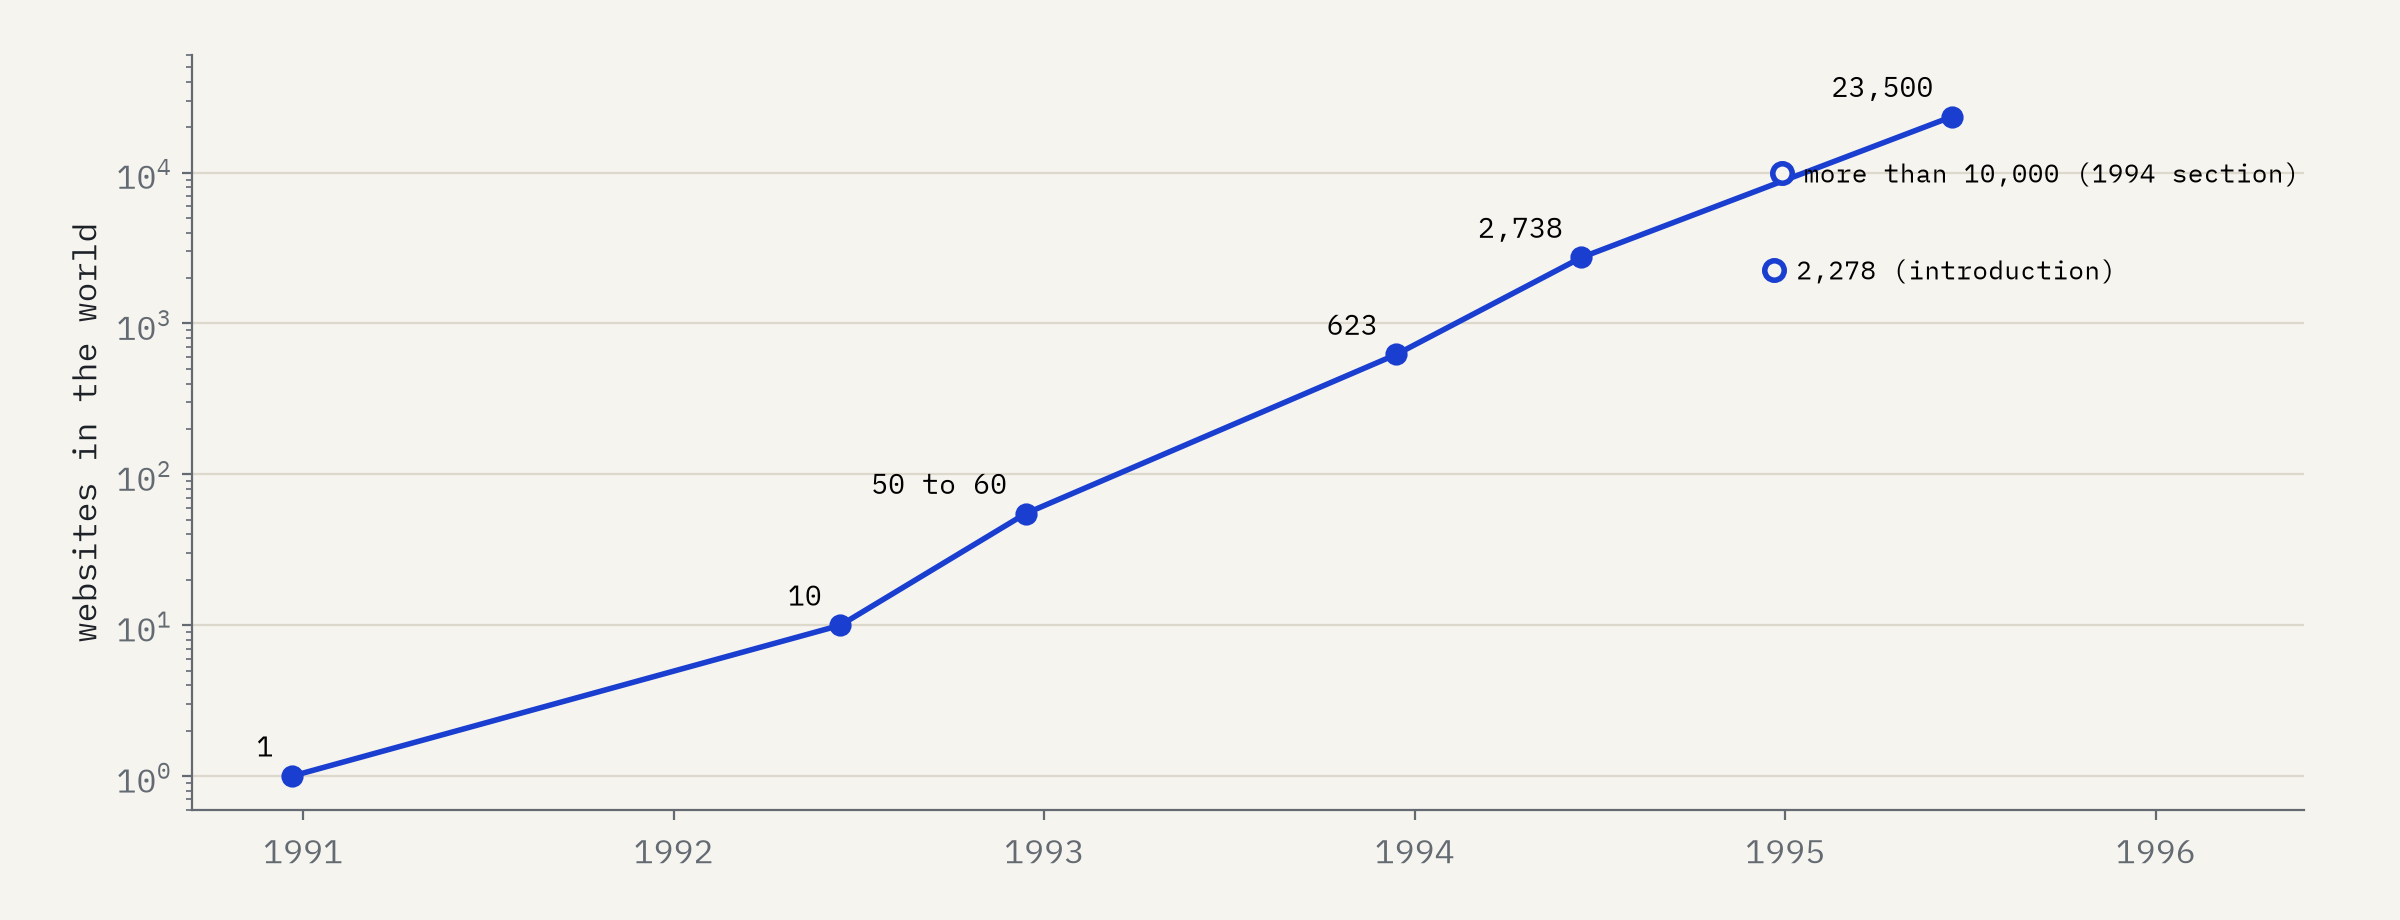
\includegraphics[width=\textwidth]{f_counts.png}
\caption{Counts of all the world's websites quoted in Wikipedia's pre-1995 list, log scale. Open circles: the two conflicting figures for the end of 1994.}\label{fig:counts}\end{figure}

\section{Methods}
\subsection{Coding the list}
I split the list on its headings into 120 entries. Chabad.org appears under both 1993 and 1994 and is counted once, in 1993, leaving 119. The year of an entry is the year section it sits in. Two exceptions are noted but not changed: the entry for Wired, under 1993, states that the site launched in October 1994; and the list dates CERN's site to 1991 while ``History of the World Wide Web'' dates info.cern.ch to 20 December 1990, which I use for the map and the country table.

For each entry I record a country and, where possible, a place. Where the paragraph names a place or a host institution (a university, a laboratory, a city) I use it (42 entries); otherwise I use the well-known home of the organisation behind the site (49); for 15 only the country is known; 13 give no indication and have no country. Each placed point is checked to fall inside its country's Natural Earth outline. I code each website into one of eight kinds (Table~\ref{tab:types}). Status is taken only from the text: an entry is ``still online'' or ``closed'' only where its paragraph says so, and the phrase that says so is checked by the code; otherwise it is ``not stated''.

\subsection{Wikidata websites}
Items are collapsed to one row each, keeping the earliest inception. An item's country is the Natural Earth country containing its headquarters coordinates where these exist (in 114 cases this overrides or replaces Wikidata's own country, for example a company domiciled in the Cayman Islands but headquartered in China), otherwise Wikidata's country. Historical states map to their main successor (the Kingdom of the Netherlands to the Netherlands, Serbia and Montenegro to Serbia). Four Usenet newsgroups typed as websites are dropped.

Inception is the weakest field. The first website went up in December 1990, so an inception before 1990 cannot be a web launch: 915 items (29.3\%) fall there, such as the Buenos Aires Herald, founded as a newspaper in 1876. I treat these as the founding of the parent organisation and leave them out, keeping 2,208 websites with an inception from 1990 to 2000. Even this floor is generous: Wikidata dates 139 websites to 1990 to 1992, more than twice the fifty to sixty that existed at the end of 1992, so most of those dates are also organisations' founding years. Regions are the United States, Europe (Natural Earth's continent, including Russia) and the rest of the world.

\subsection{The earliest recorded website in each country}
For each country I take the earliest of (a) the list's entries, with CERN dated 1990, and (b) Wikidata websites with an inception from 1993 on. The stricter floor for this one measure removes the 1990 to 1992 founding dates that would otherwise light up 35 countries before the web had reached them. Within a year, list entries and dated months come before year-only Wikidata dates. I flag, without removing, Wikidata firsts dated before the country had its own internet domain (counting predecessor domains: .su for former Soviet states, .yu for Serbia and Montenegro, .cs for the Czech Republic and Slovakia, .an for Curaçao): 5 countries (Mauritania, Cambodia, Palestine, Bosnia and Herzegovina, Rwanda).

\subsection{Domains}
Two-letter ccTLDs are matched to countries by their code (.uk for the United Kingdom); Wikidata inception is taken as the creation of the domain. 235 matched domains have a date. Where Wikipedia's table also gives a year, the two agree for 30 of 33; the disagreements are .it (1987 in Wikidata, 1988 in Wikipedia); .ma (1993 in Wikidata, 1992 in Wikipedia); .cl (1995 in Wikidata, 1987 in Wikipedia).

\begin{table}[tbp]\centering\small\caption{The pre-1995 list by kind of website (my coding): count, share, what the text says about status, and year.}\label{tab:types}\begin{tabular}{lrrrrrrr}\toprule Kind & Sites & Share & Online & Closed & 1991 to 1992 & 1993 & 1994\\\midrule
Science and research & 15 & 12.6\% & 5 & 1 & 7 & 6 & 2\\
Universities and libraries & 8 & 6.7\% & 2 & 0 & 5 & 2 & 1\\
Companies and shops & 20 & 16.8\% & 5 & 3 & 2 & 4 & 14\\
News, magazines and broadcasters & 16 & 13.4\% & 8 & 2 & 0 & 5 & 11\\
Government and politics & 10 & 8.4\% & 5 & 0 & 0 & 1 & 9\\
Search engines and directories & 10 & 8.4\% & 2 & 3 & 1 & 2 & 7\\
Culture, causes and faith & 14 & 11.8\% & 5 & 0 & 1 & 3 & 10\\
Fans, hobbies and fun & 26 & 21.8\% & 11 & 5 & 1 & 5 & 20\\
\midrule All & 119 & 100\% & 43 & 14 & 17 & 28 & 74\\
\bottomrule\end{tabular}\end{table}

\section{Results}
\subsection{The list: from laboratories to everybody}
The list grows from 3 websites in 1991 to 14 in 1992, 28 in 1993 and 74 in 1994 (Figure~\ref{fig:years}). Its earliest entries are almost all scientific: of the 17 from 1991 and 1992, 12 (70.6\%) belonged to laboratories, universities or libraries, among them CERN, SLAC (the first web server outside Europe, 12 December 1991), Fermilab, Nikhef (the third website in the world, February 1992, by the list's count), University College Cork (the first in Ireland), the Hebrew University of Jerusalem (the first written right to left) and KEK (the first web page in Japan, September 1992). By 1994 that share had fallen to 4.1\% (3 of 74). Companies, newspapers and broadcasters, government bodies, search engines and above all personal and fan sites (20 in 1994 alone; 26 in the whole list, the largest group) took over.

\begin{figure}[tbp]\centering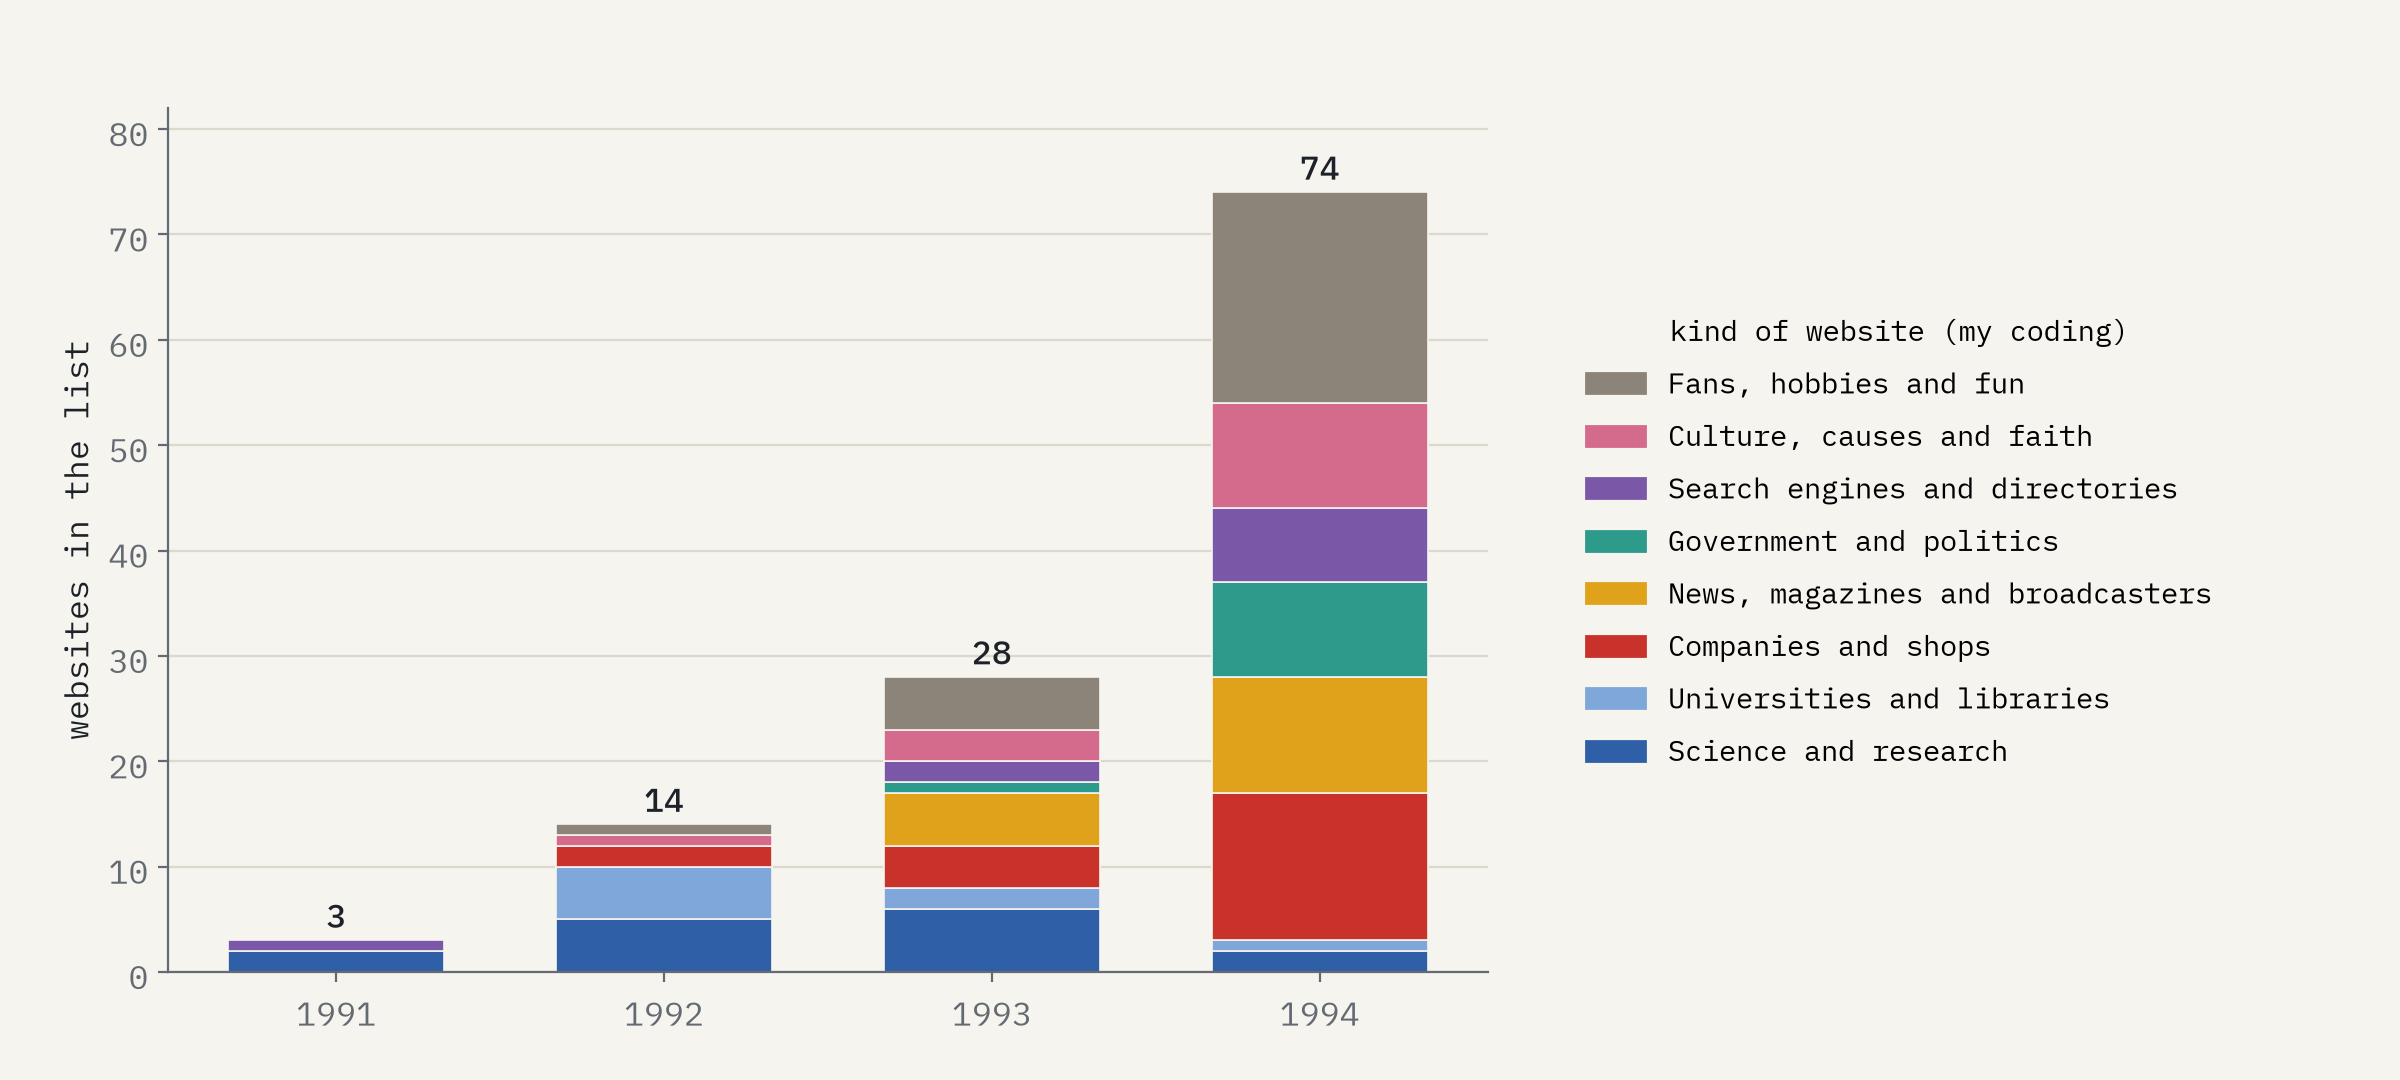
\includegraphics[width=\textwidth]{f_list_years.png}
\caption{Websites in Wikipedia's pre-1995 list, by year section and kind (my coding).}\label{fig:years}\end{figure}

The text says 43 websites (36.1\%) are still online, at the same or a new address, and 14 (11.8\%) have closed or been absorbed; for 62 (52.1\%) it is silent (Figure~\ref{fig:status}). Both counts are therefore floors. I did not check the websites themselves.

\begin{figure}[tbp]\centering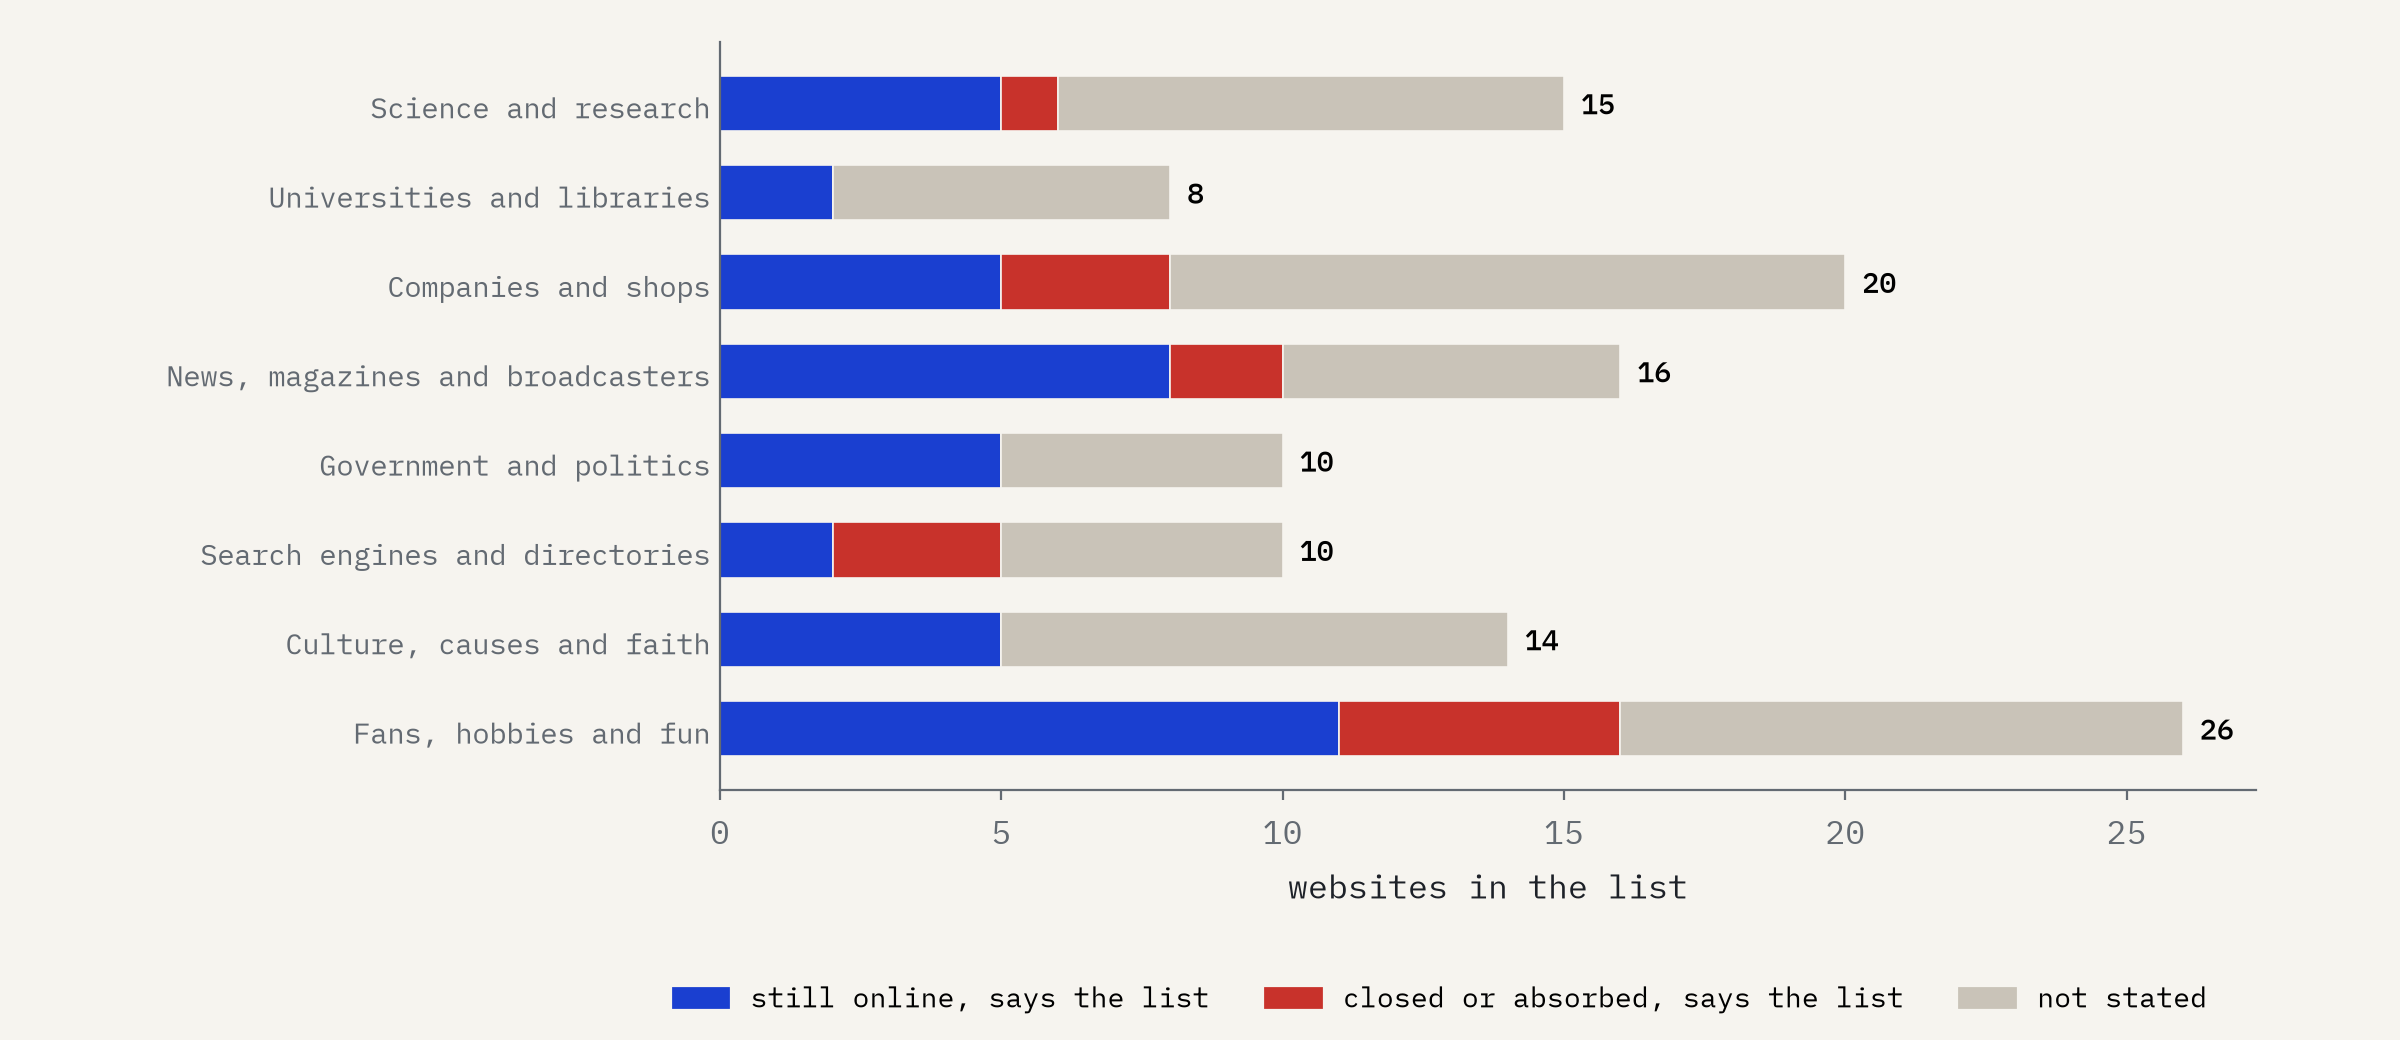
\includegraphics[width=\textwidth]{f_status.png}
\caption{Websites in the pre-1995 list by kind and by what the list's text says about them today.}\label{fig:status}\end{figure}

\subsection{Where the listed websites were}
14 countries appear in the list (Figure~\ref{fig:countries}). The United States has 74 websites, 69.8\% of the 106 that can be placed, and holds a majority of each year's placed websites from 1992 on (77.8\% in 1994). Europe has 25 (23.6\%), led by the United Kingdom (11) and Ireland (4). The remaining 7 are in Canada, Japan, Israel and Mexico. Table~\ref{tab:list} in the appendix lists every entry with its coding.

\begin{figure}[tbp]\centering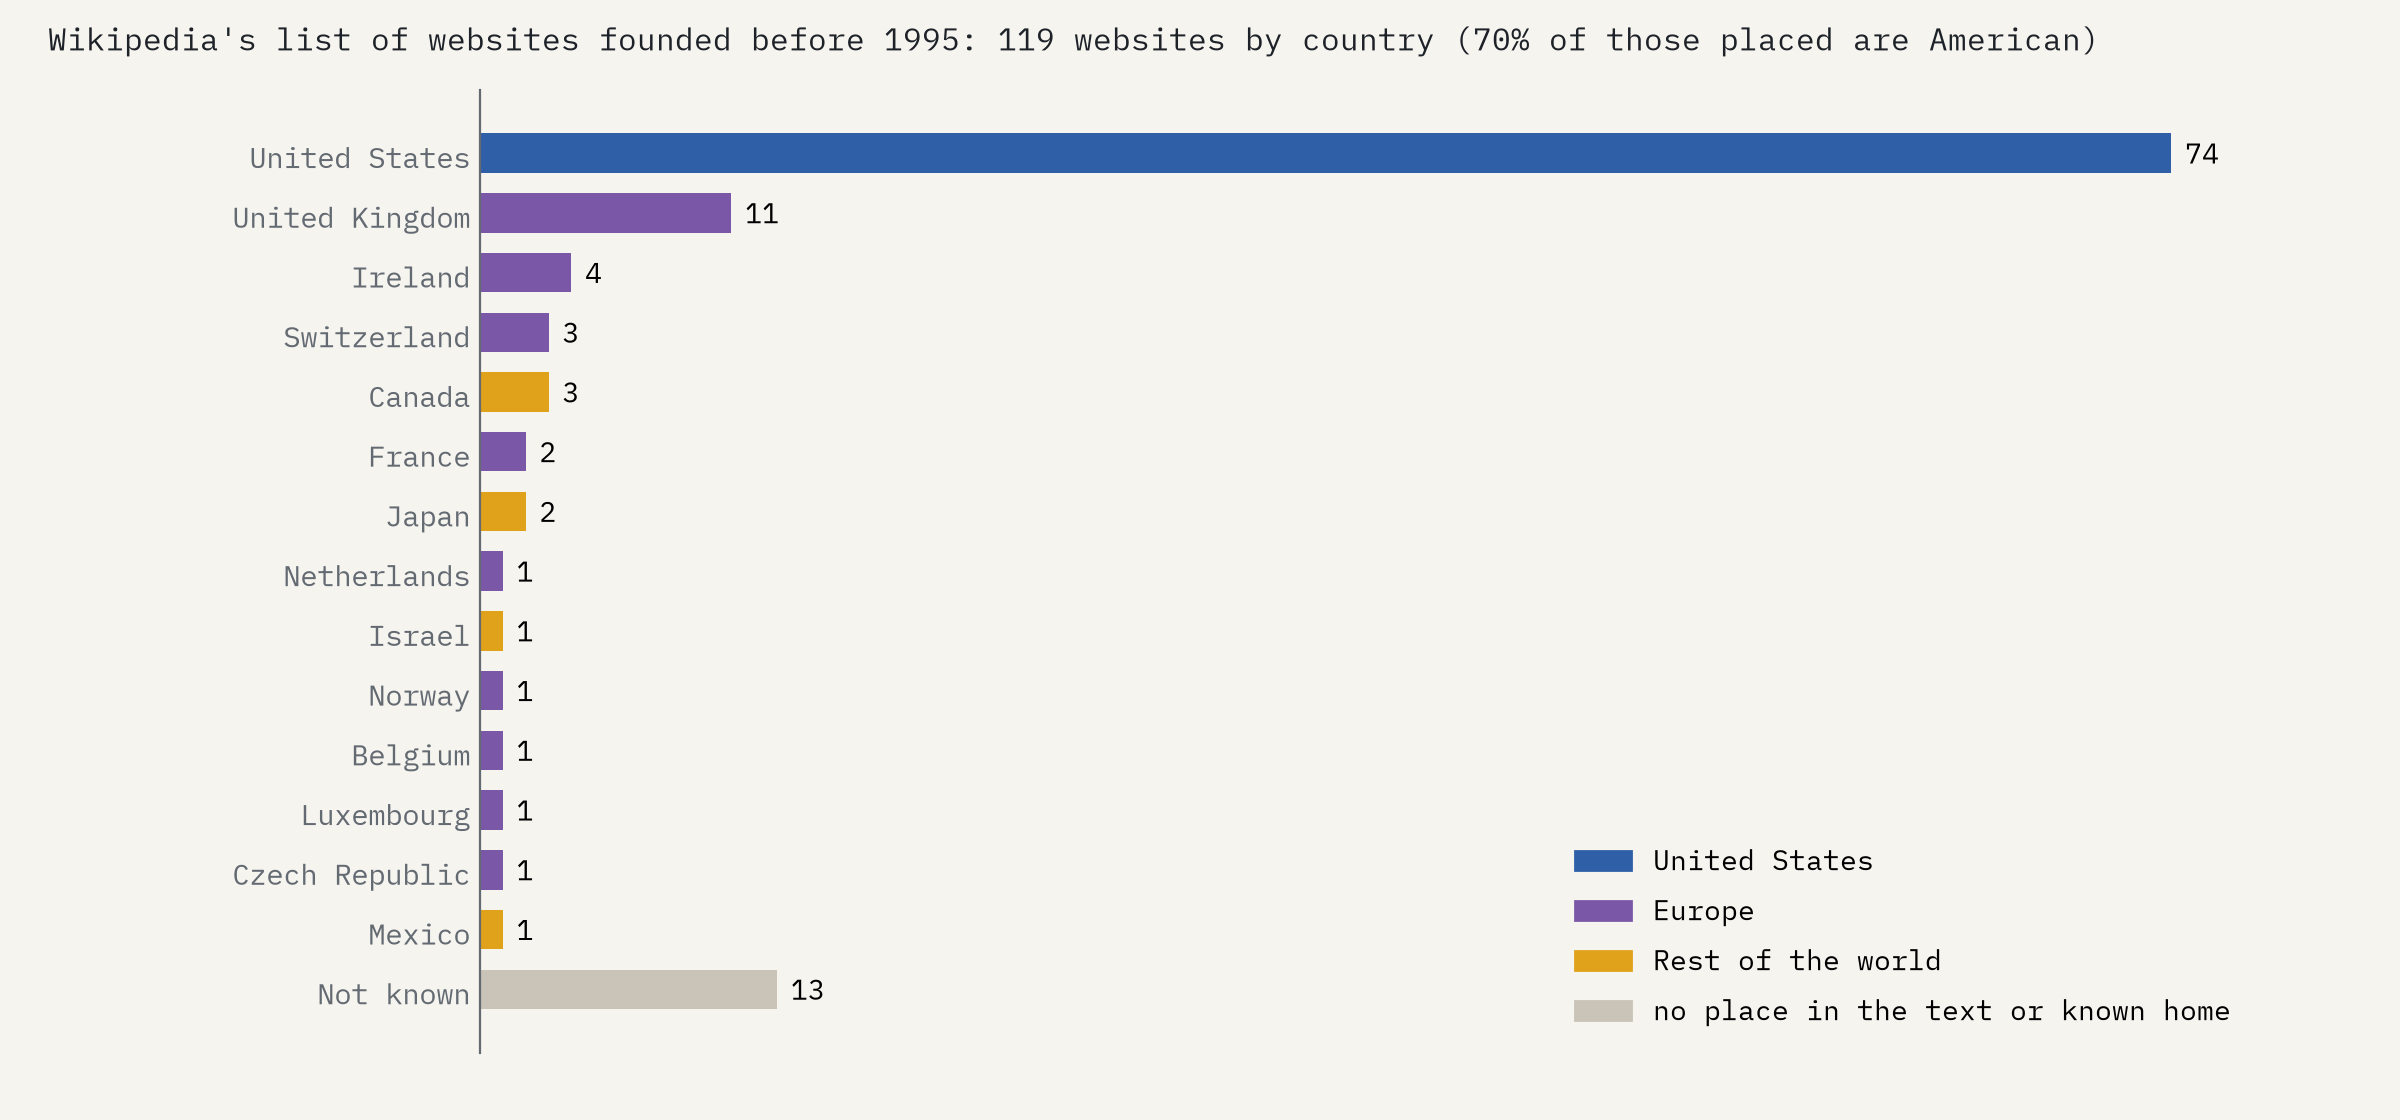
\includegraphics[width=\textwidth]{f_countries.png}
\caption{Websites in the pre-1995 list by country.}\label{fig:countries}\end{figure}

\subsection{Wikidata: the decade}
Wikidata's websites founded from 1990 to 2000 rise from 104 in 1994 to 191 in 1995 and peak at 438 in 1999; 86.3\% date from 1995 or later (Figure~\ref{fig:wd}). Coverage is thin: 58.8\% have a country, 25.5\% headquarters coordinates, 59.1\% an English Wikipedia article and 92.3\% an official address. The websites with a country are spread over 85 countries; the United States has 370, then Russia (94), the United Kingdom (87), Germany (79) and France (56).

\begin{figure}[tbp]\centering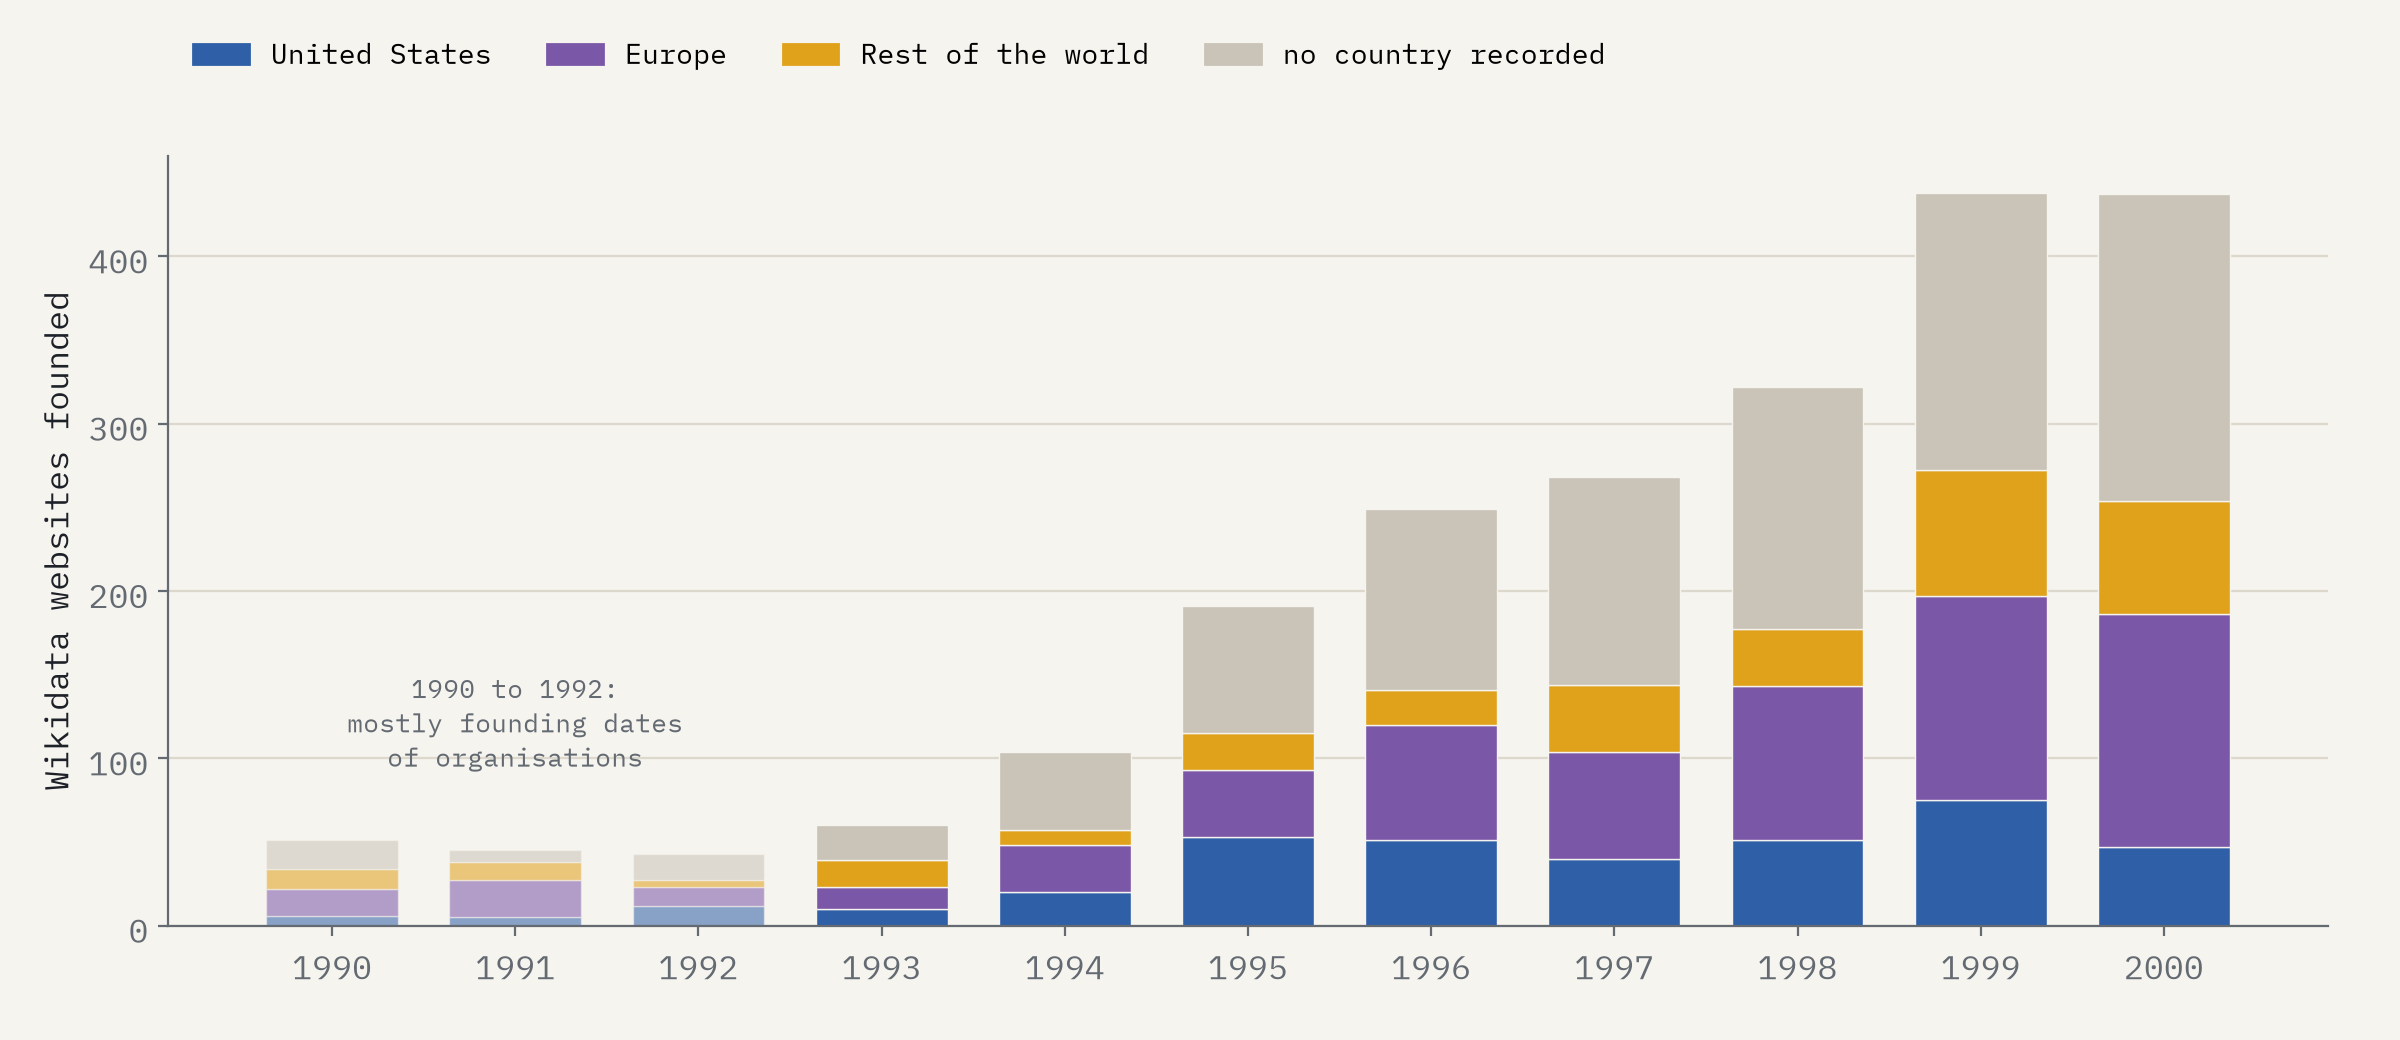
\includegraphics[width=\textwidth]{f_wd_years.png}
\caption{Wikidata websites by year of inception and region, 1990 to 2000. Faded: 1990 to 1992, years whose dates are mostly organisations' founding.}\label{fig:wd}\end{figure}

The geography is the reverse of the list's (Figure~\ref{fig:share}). Of Wikidata's websites with a country, 28.5\% are American, 47.5\% European and 24.0\% elsewhere; the American share is 27.2\% for 1990 to 1994 (195 websites) and 28.7\% for 1995 to 2000 (1,103), and swings between 13.2\% (1991) and 46.1\% (1995) in single years. Adding the 127 websites without a country whose address ends in a country code lowers it to 26.0\%. Because American websites mostly used .com, websites with no recorded country are probably more often American than the rest, so Wikidata's figure is likely an underestimate; the list, written in English and from memory, is likely an overestimate. The data cannot say where between them the truth lies.

\begin{figure}[tbp]\centering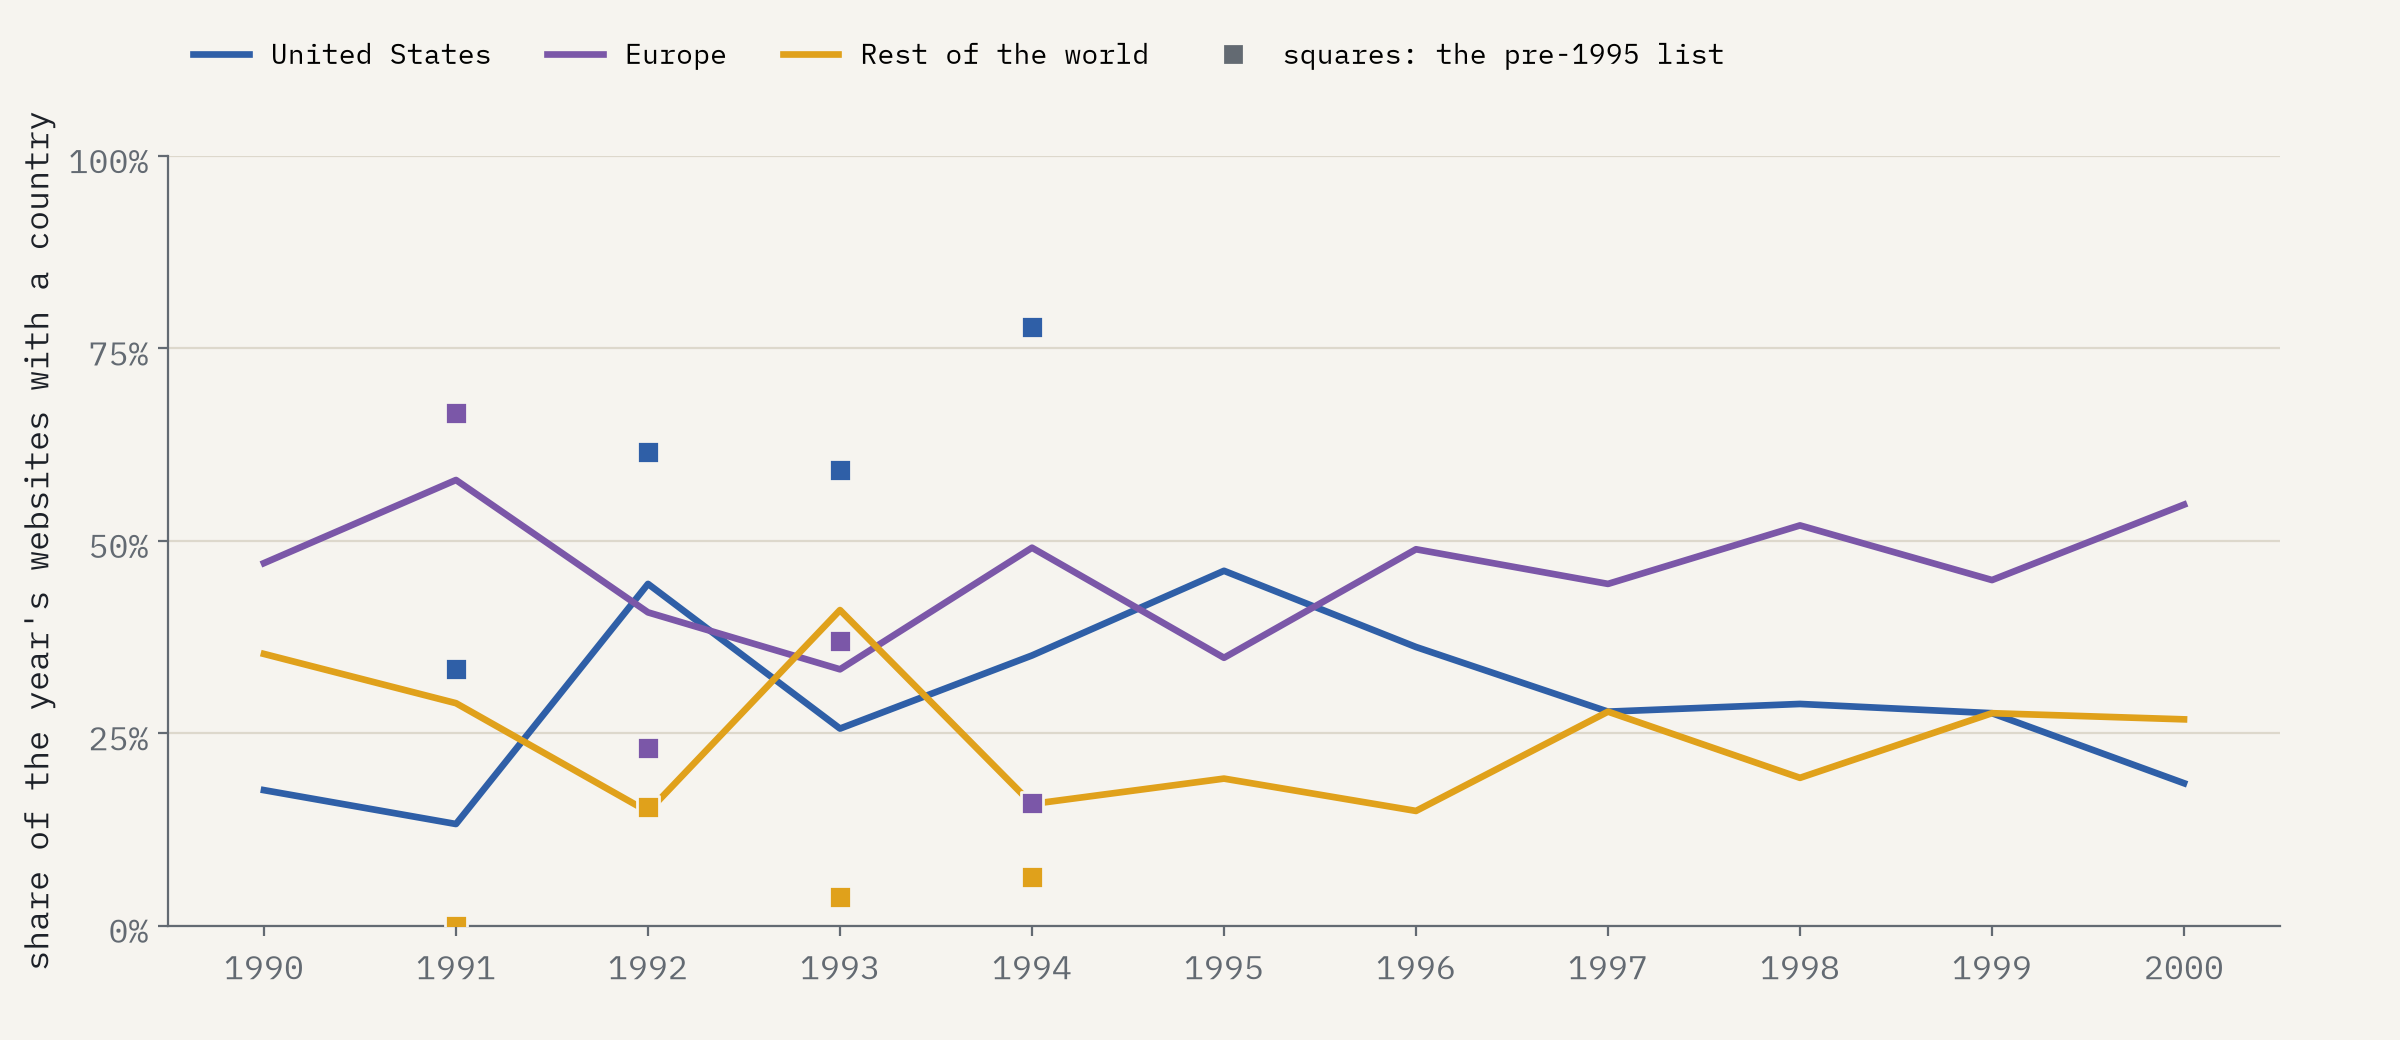
\includegraphics[width=\textwidth]{f_share.png}
\caption{Share of each year's websites with a known country by region: Wikidata (lines) and the pre-1995 list (squares).}\label{fig:share}\end{figure}

\subsection{Country by country}
Figure~\ref{fig:map} maps the earliest recorded website in each country and Table~\ref{tab:firsts} lists them. Switzerland comes first (1990) and the United States second (SLAC, December 1991). Five more join in 1992, all from the list: the Netherlands, Ireland, Israel, Japan and France. 20 countries are added in 1993, the year the web became free to use, but 20 is also where Wikidata's dates begin to count, so part of that jump is the source changing. By the end of 1994 35 countries have a recorded website and by 2000 83, home to 76.0\% of the present world population; 155 of Natural Earth's 238 countries and territories have none. Africa is least covered: 8 of its 53 countries have a record, and its earliest unflagged one is South Africa in 1995.

\begin{figure}[tbp]\centering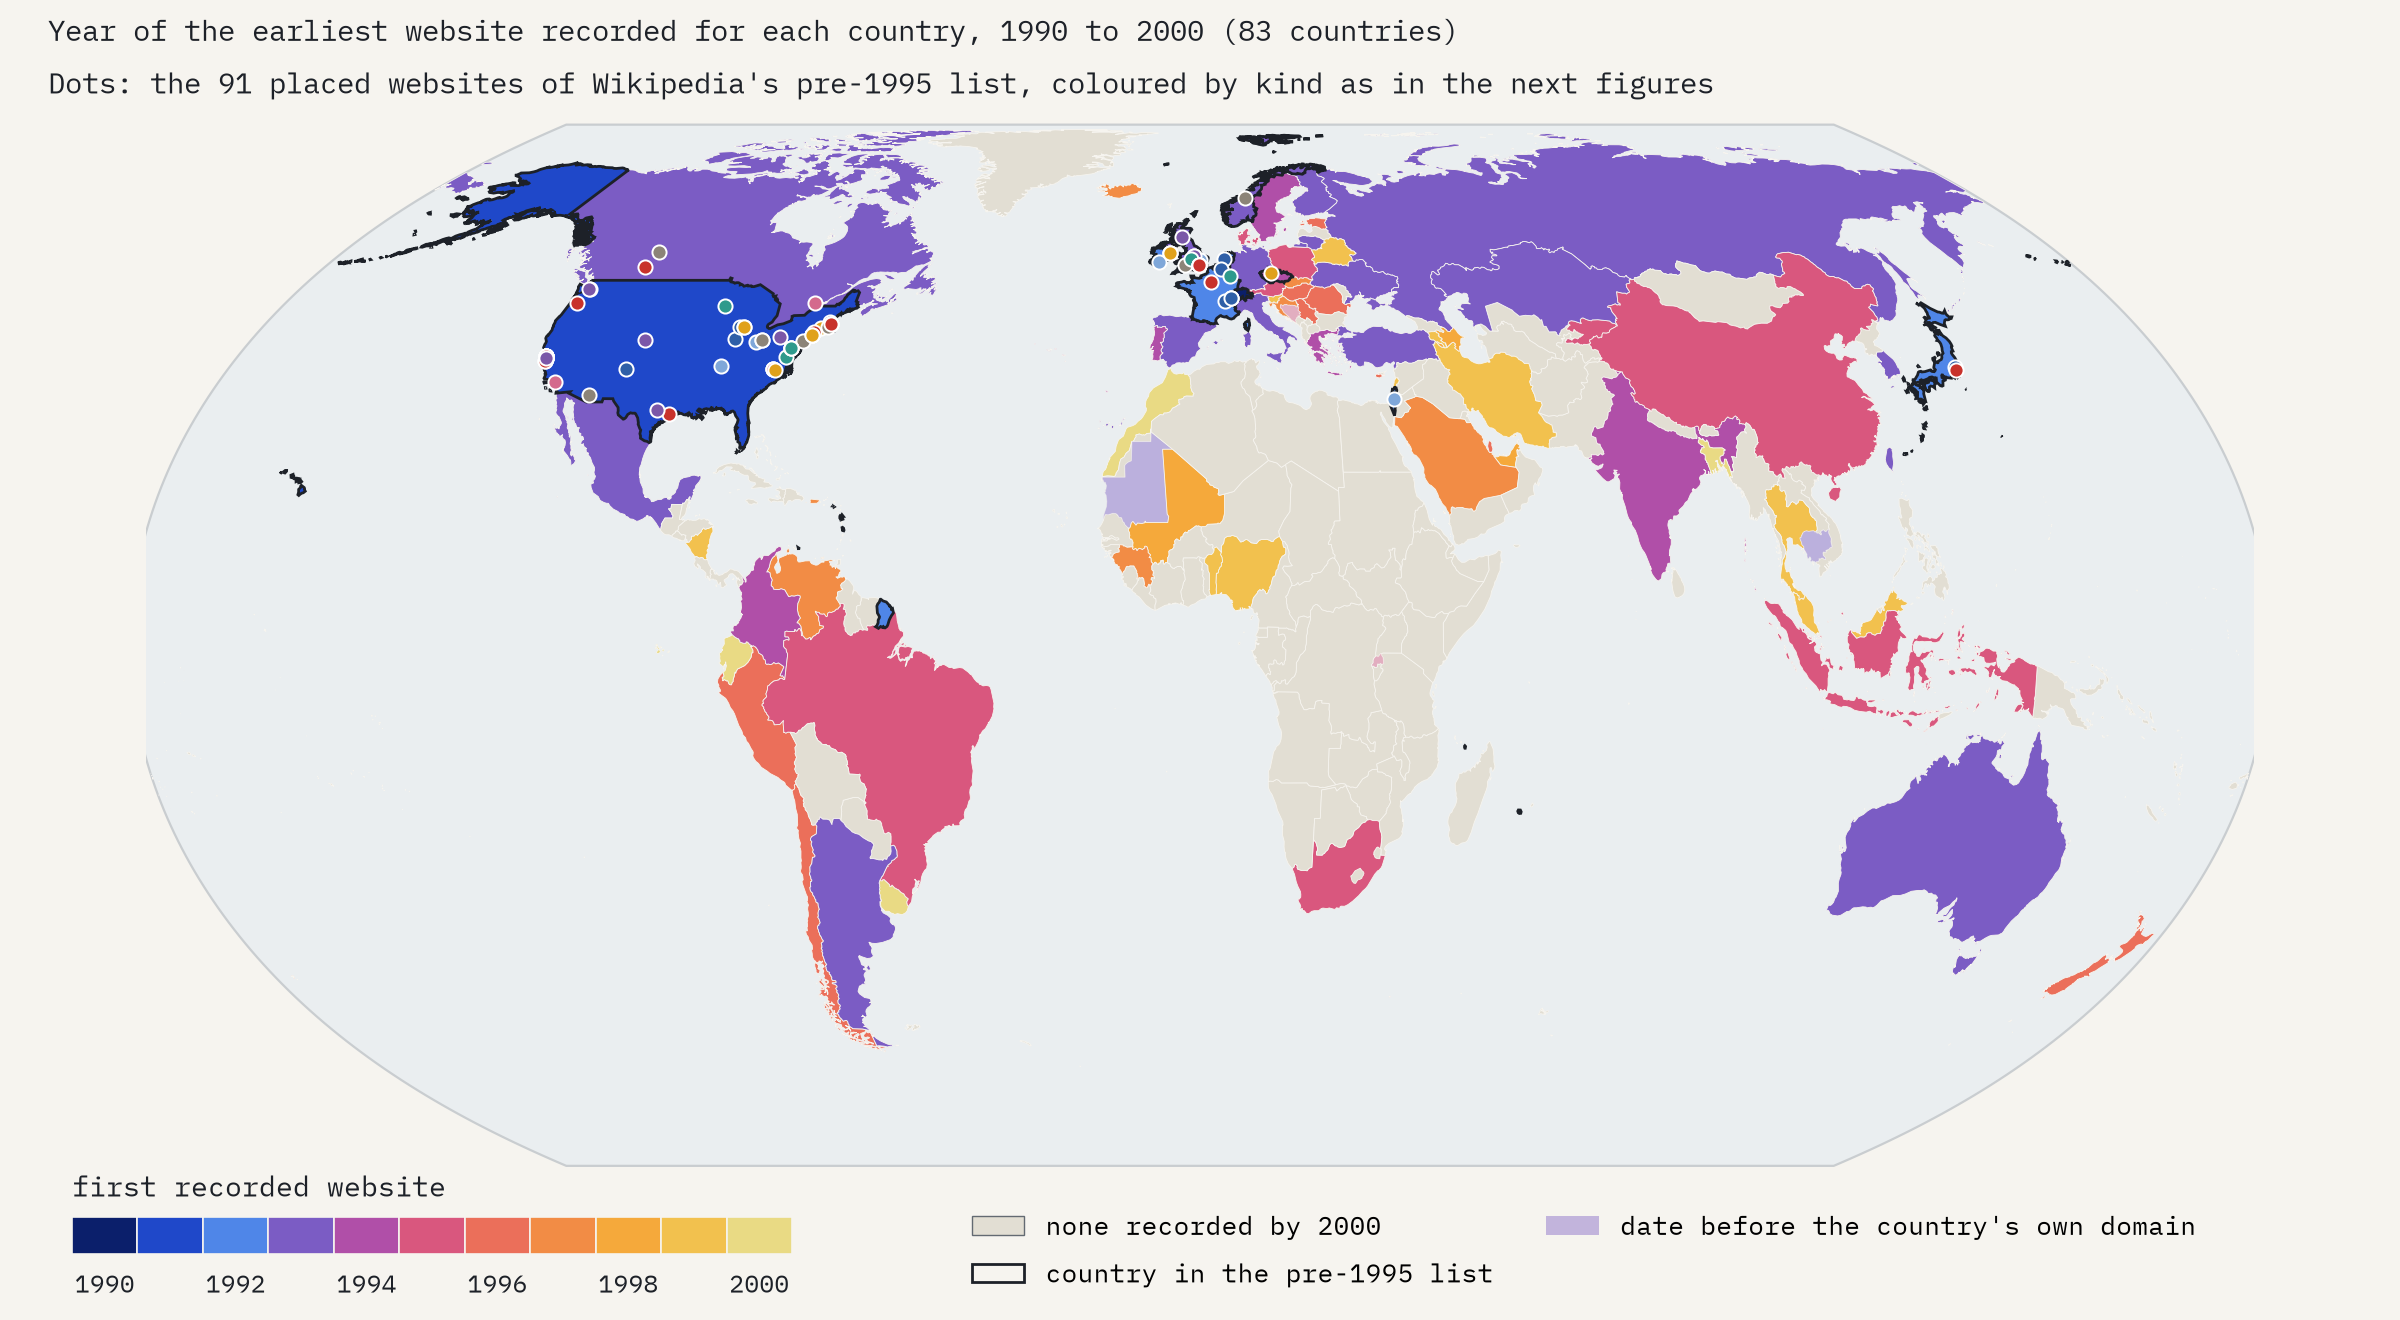
\includegraphics[width=\textwidth]{f_map.png}
\caption{Year of the earliest website recorded for each country in the pre-1995 list or (from 1993) Wikidata. Outlined: countries in the list. Faded: Wikidata dates before the country had its own domain. Dots: listed websites, coloured by kind.}\label{fig:map}\end{figure}

Domains came first (Figure~\ref{fig:spread}). 34 matched country domains existed by the end of 1989, 130 by 1994 and 223 by 2000, with the most new ones (33) in 1997. For the 12 countries whose first record comes from the list, the website followed the domain by a median of 6.0 years (range -1 to 8; Luxembourg's CORDIS, at www.cordis.lu in November 1994, predates Wikidata's 1995 date for .lu, which suggests that date is too late). Across all 83 countries the median gap is 5.0 years.

\begin{figure}[tbp]\centering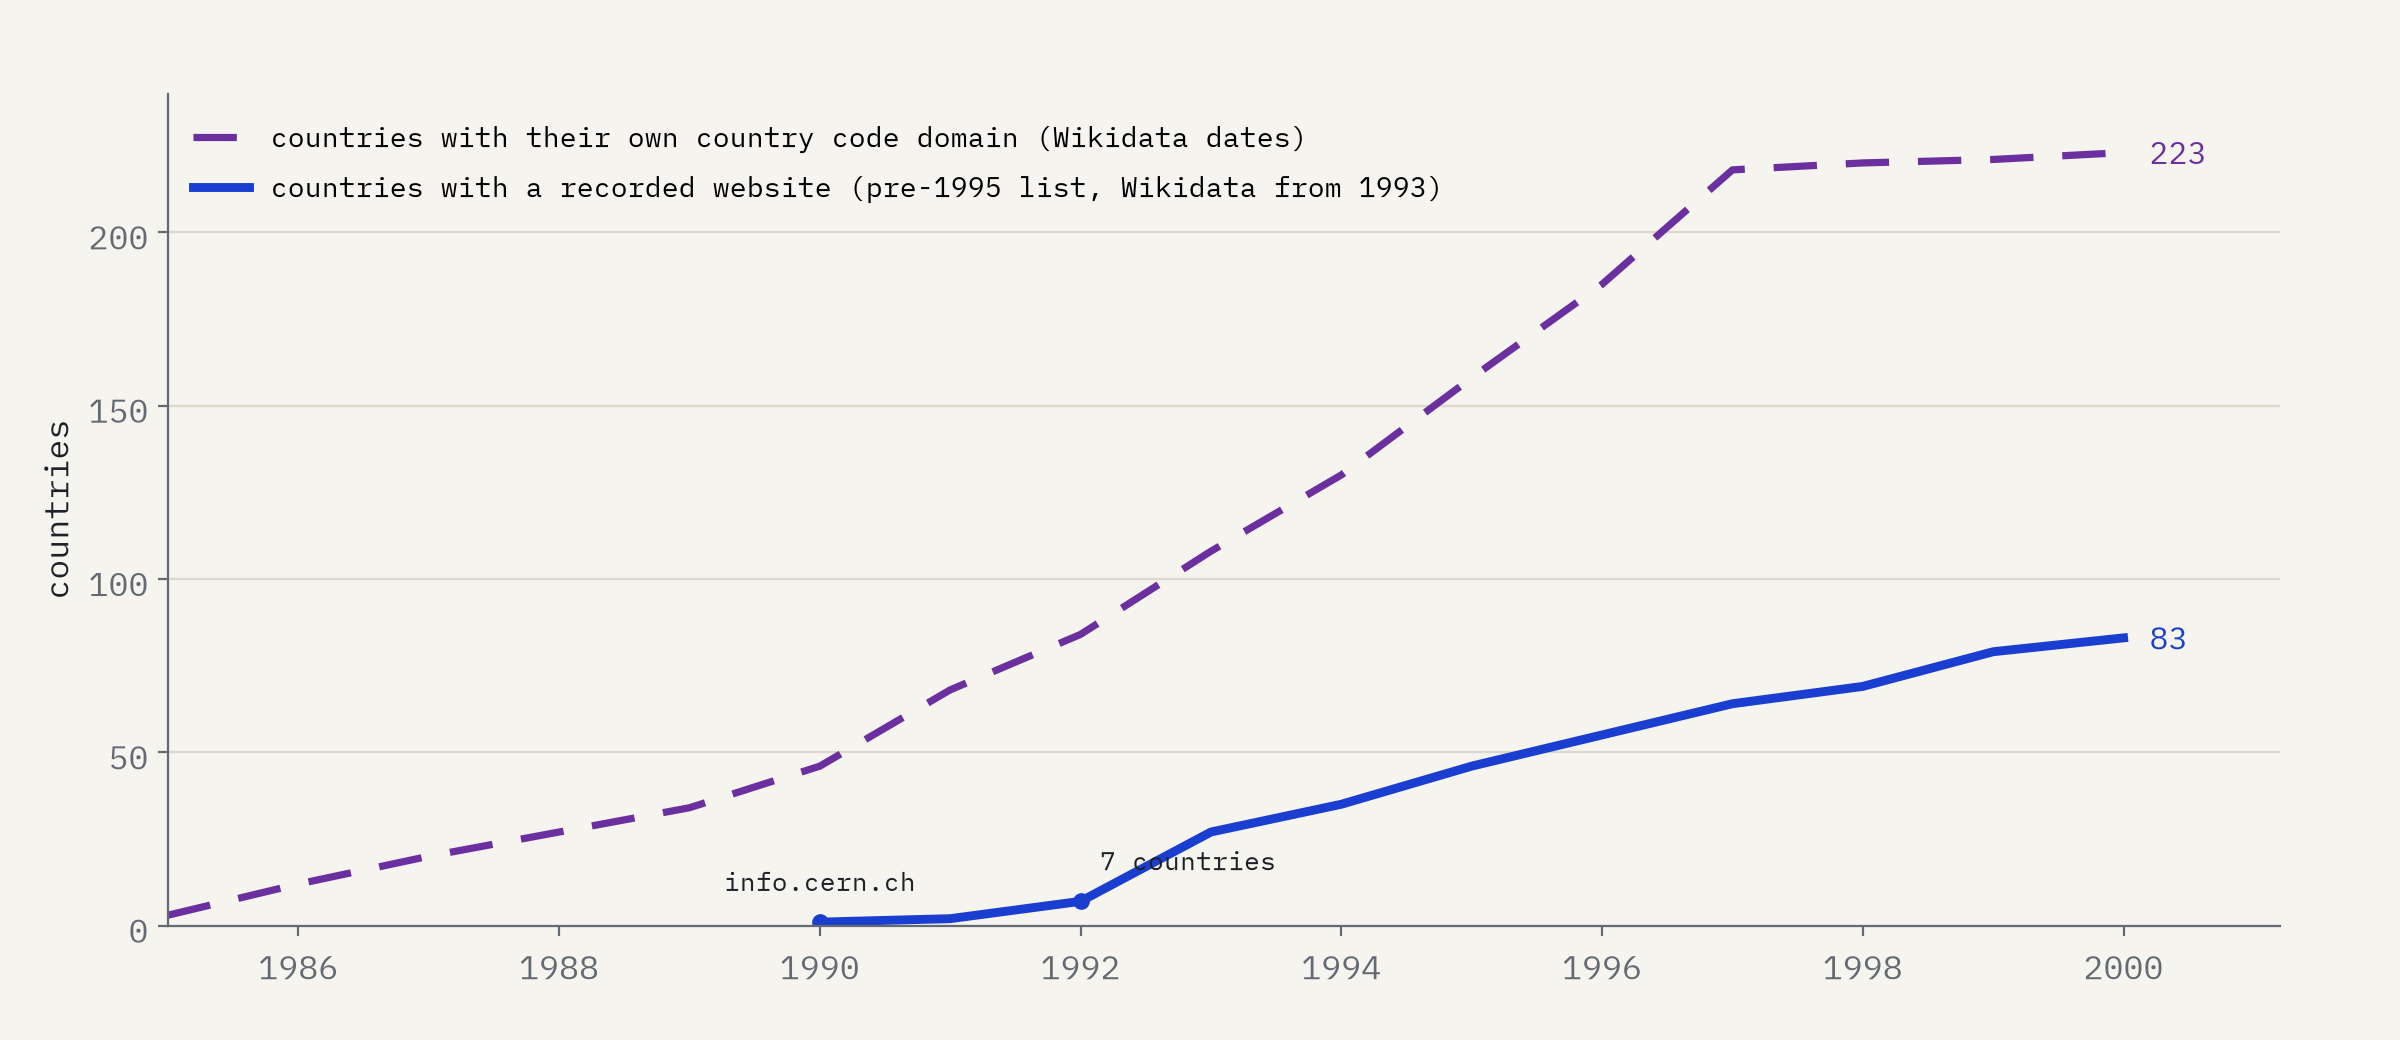
\includegraphics[width=\textwidth]{f_spread.png}
\caption{Countries with a recorded website and countries with their own country code domain, cumulative.}\label{fig:spread}\end{figure}

\section{Limitations}
First, none of the sources is a census: the list is a curated 4.1\% of pre-1995 websites, and Wikidata holds what its editors have added. Second, Wikidata's inception often records the founding of an organisation rather than of its website; the floors at 1990 and, for country firsts, 1993, and the domain flag reduce but cannot remove this. Third, the coding of the list (country, place, kind) is mine, and for 49 entries the place comes from general knowledge of the organisation rather than the text. Fourth, the list's status reflects what its editors wrote, not a check of the websites. Fifth, ``first recorded'' is first in these sources; countries surely had websites earlier than the ones recorded here. Sixth, Wikidata's domain dates are themselves imperfect, as the Luxembourg case and three disagreements with Wikipedia show.

\section{Conclusion}
The web began as a physicists' tool in Switzerland and California and within four years had become a medium for companies, newspapers, governments and fans, overwhelmingly American in the English-language memory of it. By 2000 at least 83 countries had a website on record. The sources that let us see this are uneven: Wikipedia's list remembers the American web; Wikidata remembers much more of Europe's and the rest of the world's, but with dates that often belong to the organisations, not the sites. Read together, and with their limits in view, they show how quickly the web spread, and how much of its early history has not been written down.

\section*{Data and code availability}
The interactive map is at \url{https://maps.tristanhotham.com/first-websites/}. Data and code are at \url{https://github.com/Tristan-Hotham/first-websites} and archived with this paper at https://doi.org/10.5281/zenodo.23878602. Derived data are released under CC BY 4.0 and code under the MIT licence. Wikipedia content is CC BY-SA 4.0; Wikidata is CC0.

\section*{AI statement}
I wrote the text, with drafting and editing assistance from Claude (Anthropic), which also helped prepare the analysis code. I reviewed and checked all text and results.

\begin{thebibliography}{9}
\bibitem[Natural Earth(2026)]{naturalearth} Natural Earth (2026) Admin 0 countries and populated places, 1:50m and 1:10m. Public domain. \url{https://www.naturalearthdata.com/}
\bibitem[Wikidata(2026)]{wikidata} Wikidata contributors (2026) Websites (Q35127 and subclasses) and country code top-level domains (Q42032), queried through QLever. CC0. \url{https://www.wikidata.org/}
\bibitem[Wikipedia(2026a)]{wikilist} Wikipedia contributors (2026) List of websites founded before 1995 (revision 1382290598). CC BY-SA 4.0. \url{https://en.wikipedia.org/wiki/List_of_websites_founded_before_1995}
\bibitem[Wikipedia(2026b)]{wikihist} Wikipedia contributors (2026) History of the World Wide Web (revision 1383306370). CC BY-SA 4.0. \url{https://en.wikipedia.org/wiki/History_of_the_World_Wide_Web}
\bibitem[Wikipedia(2026c)]{wikicc} Wikipedia contributors (2026) Country code top-level domain (revision 1382234250). CC BY-SA 4.0. \url{https://en.wikipedia.org/wiki/Country_code_top-level_domain}
\bibitem[Wikipedia(2026d)]{wikitld} Wikipedia contributors (2026) List of Internet top-level domains (revision 1383138271). CC BY-SA 4.0. \url{https://en.wikipedia.org/wiki/List_of_Internet_top-level_domains}
\end{thebibliography}

\clearpage
\appendix
\section{The earliest recorded website in each country}
\begin{small}\begin{longtable}{lrp{6.2cm}ll}\caption{Earliest recorded website in each country. ? = dated before the country's own domain. Last column: country code domain and its Wikidata year.}\label{tab:firsts}\\\toprule Country & Year & Website & Source & Domain\\\midrule\endfirsthead\toprule Country & Year & Website & Source & Domain\\\midrule\endhead
Switzerland & 1990 & CERN & list & .ch 1987\\
United States & 1991 & Stanford Linear Accelerator Center & list & .us 1985\\
Netherlands & 1992 & Nikhef & list & .nl 1986\\
Ireland & 1992 & CURIA & list & .ie 1988\\
Israel & 1992 & HUJI & list & .il 1985\\
Japan & 1992 & KEK & list & .jp 1986\\
France & 1992 & IN2P3 & list & .fr 1986\\
Ukraine & 1993 & Ukrainian Independent Information Agency & Wikidata & .ua 1992\\
Argentina & 1993 & A24 & Wikidata & .ar 1987\\
Germany & 1993 & The Patches Scrolls & Wikidata & .de 1986\\
Russia & 1993 & Novaya Gazeta & Wikidata & .ru 1994\\
South Korea & 1993 & Maeil Labor News & Wikidata & .kr 1986\\
Belgium & 1993 & Principia Cybernetica & list & .be 1988\\
Mauritania & 1993? & Le Calame & Wikidata & .mr 1996\\
Mexico & 1993 & Siglo de Durango & Wikidata & .mx 1989\\
Spain & 1993 & Cajadecarton.es & Wikidata & .es 1988\\
Canada & 1993 & Flags of the World & Wikidata & .ca 1987\\
Finland & 1993 & Kokkolan Halpa-Halli Oy & Wikidata & .fi 1986\\
Taiwan & 1993 & 104 Job Bank & Wikidata & .tw 1989\\
Norway & 1993 & Joachim Jarre Society & list & .no 1987\\
United Kingdom & 1993 & Trojan Room coffee pot & list & .uk 1985\\
Australia & 1993 & Doongal Aboriginal Art & Wikidata & .au 1986\\
Cambodia & 1993? & The Cambodia Daily & Wikidata & .kh 1996\\
Italy & 1993 & Patrizia Pepe & Wikidata & .it 1987\\
Kazakhstan & 1993 & ALAU.KZ & Wikidata & .kz 1994\\
Lithuania & 1993 & Mano namai & Wikidata & .lt 1992\\
Turkey & 1993 & TGRT Haber & Wikidata & .tr 1990\\
Greece & 1994 & Sportime & Wikidata & .gr 1989\\
Colombia & 1994 & La Nación & Wikidata & .co 1991\\
Luxembourg & 1994 & CORDIS & list & .lu 1995\\
Czech Republic & 1994 & Radio Prague & list & .cz 1993\\
India & 1994 & India TV & Wikidata & .in 1989\\
Palestine & 1994? & Snunit & Wikidata & .ps 2000\\
Portugal & 1994 & Motociclismo & Wikidata & .pt 1988\\
Sweden & 1994 & Yelah & Wikidata & .se 1986\\
Austria & 1995 & derStandard.at & Wikidata & .at 1988\\
Hong Kong & 1995 & Weather Underground of Hong Kong & Wikidata & .hk 1990\\
Denmark & 1995 & Scope & Wikidata & .dk 1987\\
China & 1995 & Dahe Daily & Wikidata & .cn 1990\\
Bosnia and Herzegovina & 1995? & Commission to Preserve National Monuments of B & Wikidata & .ba 1996\\
Brazil & 1995 & Shoptime & Wikidata & .br 1989\\
Indonesia & 1995 & Tempo.co & Wikidata & .id 1993\\
Kyrgyzstan & 1995 & Neman-Pharm & Wikidata & .kg 1995\\
Poland & 1995 & Wirtualna Polska & Wikidata & .pl 1990\\
Rwanda & 1995? & The New Times & Wikidata & .rw 1996\\
South Africa & 1995 & Design Indaba & Wikidata & .za 1990\\
Romania & 1996 & cIMeC.Ro & Wikidata & .ro 1993\\
New Zealand & 1996 & Jasons Travel Media & Wikidata & .nz 1987\\
Serbia & 1996 & Blic & Wikidata & .rs 2008\\
Estonia & 1996 & NETI & Wikidata & .ee 1992\\
Qatar & 1996 & Al Jazeera & Wikidata & .qa 1996\\
Chile & 1996 & Gob.cl & Wikidata & .cl 1995\\
Cyprus & 1996 & Robtex & Wikidata & .cy 1994\\
Hungary & 1996 & Web Gallery of Art & Wikidata & .hu 1990\\
Peru & 1996 & Ciberayllu & Wikidata & .pe 1991\\
Cayman Islands & 1997 & NetEase & Wikidata & .ky 1995\\
Croatia & 1997 & Monitor.hr & Wikidata & .hr 1993\\
Curaçao & 1997 & GoldenPalace.com & Wikidata & .cw 2010\\
Guinea & 1997 & Guinéenews & Wikidata & .gn 1994\\
Iceland & 1997 & Kvikmyndir & Wikidata & .is 1986\\
Puerto Rico & 1997 & Primera Hora & Wikidata & .pr 1989\\
Saudi Arabia & 1997 & Islam Questions \& Answers & Wikidata & .sa 1994\\
Slovakia & 1997 & zoznam.sk & Wikidata & .sk 1993\\
Venezuela & 1997 & El sitio & Wikidata & .ve 1991\\
Azerbaijan & 1998 & president.az & Wikidata & .az 1993\\
Jersey & 1998 & Rakuten.co.uk & Wikidata & .je 1996\\
Mali & 1998 & aBamako & Wikidata & .ml 1993\\
Singapore & 1998 & Agoda & Wikidata & .sg 1988\\
United Arab Emirates & 1998 & Maktoob & Wikidata & .ae 1992\\
Malaysia & 1999 & Harakahdaily & Wikidata & .my 1987\\
Belarus & 1999 & kosht.com & Wikidata & .by 1994\\
Lebanon & 1999 & Al-Ahed & Wikidata & .lb 1993\\
Armenia & 1999 & Mediamax news agency & Wikidata & .am 1994\\
Benin & 1999 & Fraternité & Wikidata & .bj 1996\\
Iran & 1999 & Gamapack & Wikidata & .ir 1994\\
Nicaragua & 1999 & La Nueva Radio YA & Wikidata & .ni 1989\\
Nigeria & 1999 & Kogi State University Library & Wikidata & .ng 1995\\
Slovenia & 1999 & Bolha.com & Wikidata & .si 1993\\
Thailand & 1999 & MThai & Wikidata & .th 1988\\
Bangladesh & 2000 & bdjobs.com & Wikidata & .bd 1999\\
Ecuador & 2000 & QuitoGay.net & Wikidata & .ec 1991\\
Morocco & 2000 & Mabooko & Wikidata & .ma 1993\\
Uruguay & 2000 & La Onda Digital & Wikidata & .uy 1990\\
\bottomrule\end{longtable}\end{small}

\section{The pre-1995 list as coded}
\begin{footnotesize}\begin{longtable}{p{4.6cm}rp{2.8cm}p{4.3cm}l}\caption{Wikipedia's list of websites founded before 1995 as coded here: year section, country, kind and status in the text.}\label{tab:list}\\\toprule Website & Year & Country & Kind & Status\\\midrule\endfirsthead\toprule Website & Year & Country & Kind & Status\\\midrule\endhead
CERN & 1991 & Switzerland & Science and research & not stated\\
World Wide Web Virtual Library & 1991 & Switzerland & Search engines and directories & not stated\\
Stanford Linear Accelerator Center & 1991 & United States & Science and research & not stated\\
Nikhef & 1992 & Netherlands & Science and research & not stated\\
National Center for Supercomputing Appli & 1992 & United States & Science and research & not stated\\
FNAL & 1992 & United States & Science and research & not stated\\
SunSITE & 1992 & United States & Universities and libraries & not stated\\
Wright State University Libraries & 1992 & United States & Universities and libraries & not stated\\
Ohio State University & 1992 & United States & Universities and libraries & not stated\\
IN2P3 & 1992 & France & Science and research & not stated\\
CURIA & 1992 & Ireland & Universities and libraries & online\\
HUJI & 1992 & Israel & Universities and libraries & not stated\\
The Exploratorium & 1992 & United States & Culture, causes and faith & not stated\\
simianpress & 1992 & not known & Companies and shops & closed\\
CBSS & 1992 & United States & Companies and shops & online\\
KEK & 1992 & Japan & Science and research & online\\
Cybergrass & 1992 & United States & Fans, hobbies and fun & online\\
Bloomberg.com & 1993 & United States & News, magazines and broadcasters & not stated\\
Chabad.org & 1993 & United States & Culture, causes and faith & not stated\\
Doctor Fun & 1993 & United States & Fans, hobbies and fun & not stated\\
Électricité de France & 1993 & France & Companies and shops & not stated\\
Global Network Navigator & 1993 & United States & Search engines and directories & not stated\\
Haystack Observatory & 1993 & United States & Science and research & online\\
IMDb & 1993 & United Kingdom & Fans, hobbies and fun & not stated\\
Internet Underground Music Archive & 1993 & United States & Culture, causes and faith & not stated\\
IONA Technologies & 1993 & Ireland & Companies and shops & not stated\\
Joachim Jarre Society & 1993 & Norway & Fans, hobbies and fun & not stated\\
JumpStation & 1993 & United Kingdom & Search engines and directories & closed\\
LANL preprint archive & 1993 & United States & Science and research & online\\
LSD.com & 1993 & not known & Fans, hobbies and fun & not stated\\
The OTIS Project & 1993 & United States & Culture, causes and faith & online\\
The Tech & 1993 & United States & News, magazines and broadcasters & not stated\\
NASA & 1993 & United States & Government and politics & not stated\\
Nexor & 1993 & United Kingdom & Companies and shops & not stated\\
MTV & 1993 & United States & News, magazines and broadcasters & online\\
Nippon Telegraph and Telephone & 1993 & Japan & Companies and shops & online\\
PARC Map Server & 1993 & United States & Science and research & not stated\\
PARC Researcher & 1993 & United States & Science and research & closed\\
photo.net & 1993 & United States & Fans, hobbies and fun & not stated\\
Principia Cybernetica & 1993 & Belgium & Science and research & not stated\\
School of Mathematics, Trinity College D & 1993 & Ireland & Universities and libraries & not stated\\
ExPASy & 1993 & Switzerland & Science and research & online\\
Trojan Room coffee pot & 1993 & United Kingdom & Universities and libraries & not stated\\
Trincoll Journal & 1993 & United States & News, magazines and broadcasters & closed\\
Wired.com & 1993 & United States & News, magazines and broadcasters & online\\
ALIWEB & 1994 & United Kingdom & Search engines and directories & closed\\
Allied Artists Entertainment Group & 1994 & United States & Companies and shops & not stated\\
American Marketing Association & 1994 & United States & Culture, causes and faith & online\\
Amnesty International Canada & 1994 & Canada & Culture, causes and faith & online\\
Apple Inc. & 1994 & United States & Companies and shops & not stated\\
Art.Net & 1994 & United States & Culture, causes and faith & not stated\\
Art Crimes & 1994 & United States & Culture, causes and faith & not stated\\
The Amazing FishCam & 1994 & United States & Fans, hobbies and fun & closed\\
Automatic Complaint-Letter Generator & 1994 & United States & Fans, hobbies and fun & online\\
The Barney Fun Page & 1994 & Canada & Fans, hobbies and fun & online\\
BBC Online & 1994 & United Kingdom & News, magazines and broadcasters & online\\
Bianca's Smut Shack & 1994 & United States & Fans, hobbies and fun & not stated\\
Birmingham City Council & 1994 & United Kingdom & Government and politics & online\\
Britannica Online & 1994 & United States & News, magazines and broadcasters & online\\
Buzzweb.com & 1994 & not known & Culture, causes and faith & not stated\\
CDNAir.ca & 1994 & Canada & Companies and shops & not stated\\
CitySites & 1994 & United States & Companies and shops & online\\
Classical MIDI Archives & 1994 & not known & Culture, causes and faith & online\\
Cool Site of the Day & 1994 & United States & Search engines and directories & closed\\
Cybersell & 1994 & United States & Companies and shops & closed\\
CORDIS & 1994 & Luxembourg & Government and politics & online\\
Dianne Feinstein & 1994 & United States & Government and politics & not stated\\
The Economist & 1994 & United Kingdom & News, magazines and broadcasters & online\\
e-democracy & 1994 & United States & Government and politics & not stated\\
Einet Galaxy & 1994 & United States & Search engines and directories & online\\
FogCam! & 1994 & United States & Fans, hobbies and fun & online\\
FolkBook & 1994 & United States & Fans, hobbies and fun & closed\\
Flags of the World & 1994 & not known & Fans, hobbies and fun & online\\
GeneNetwork & 1994 & United States & Science and research & not stated\\
HM Treasury & 1994 & United Kingdom & Government and politics & online\\
Horror & 1994 & not known & Fans, hobbies and fun & online\\
HotWired & 1994 & United States & News, magazines and broadcasters & not stated\\
IBM & 1994 & United States & Companies and shops & online\\
Innerviews & 1994 & not known & News, magazines and broadcasters & online\\
The Irish Times & 1994 & Ireland & News, magazines and broadcasters & online\\
Lawinfo & 1994 & United States & Companies and shops & online\\
Legislative Information System & 1994 & United States & Government and politics & online\\
Links from the Underground & 1994 & United States & Fans, hobbies and fun & online\\
Literary Kicks & 1994 & United States & Culture, causes and faith & online\\
Lycos & 1994 & United States & Search engines and directories & online\\
Megadeth, Arizona & 1994 & United States & Culture, causes and faith & not stated\\
Microsoft & 1994 & United States & Companies and shops & not stated\\
Museum of Bad Art & 1994 & United States & Culture, causes and faith & not stated\\
The Nine Planets & 1994 & United States & Fans, hobbies and fun & online\\
Nando.net & 1994 & United States & News, magazines and broadcasters & not stated\\
NetBoy & 1994 & not known & Fans, hobbies and fun & online\\
Netrek & 1994 & United States & Fans, hobbies and fun & closed\\
Pathfinder.com & 1994 & United States & News, magazines and broadcasters & closed\\
Phish.net & 1994 & United States & Fans, hobbies and fun & not stated\\
PizzaNet & 1994 & United States & Companies and shops & not stated\\
Powells.com & 1994 & United States & Companies and shops & not stated\\
PrimePages & 1994 & United States & Universities and libraries & online\\
Purple.com & 1994 & not known & Fans, hobbies and fun & closed\\
Radio Prague & 1994 & Czech Republic & News, magazines and broadcasters & online\\
Ren and Stimpy Information & 1994 & not known & Fans, hobbies and fun & not stated\\
Senator Edward Kennedy & 1994 & United States & Government and politics & online\\
Saccharomyces Genome Database & 1994 & United States & Science and research & online\\
Sex.com & 1994 & United States & Companies and shops & not stated\\
The Skeptic's Dictionary & 1994 & United States & Fans, hobbies and fun & online\\
The Simpsons Archive & 1994 & not known & Fans, hobbies and fun & online\\
Sirius Connections & 1994 & United States & Companies and shops & not stated\\
Snopes & 1994 & United States & Fans, hobbies and fun & not stated\\
SpinnWebe & 1994 & not known & Fans, hobbies and fun & not stated\\
Telegraph.co.uk & 1994 & United Kingdom & News, magazines and broadcasters & not stated\\
United States Department of State & 1994 & United States & Government and politics & not stated\\
VeloNews & 1994 & United States & News, magazines and broadcasters & not stated\\
VirtuMall & 1994 & United States & Companies and shops & closed\\
WWW Useless Pages & 1994 & not known & Fans, hobbies and fun & closed\\
WebCrawler & 1994 & United States & Search engines and directories & not stated\\
Webmedia & 1994 & United Kingdom & Companies and shops & not stated\\
Whitehouse.gov & 1994 & United States & Government and politics & not stated\\
World-Wide Web Worm & 1994 & United States & Search engines and directories & not stated\\
Yahoo! & 1994 & United States & Search engines and directories & not stated\\
Zapatista National Liberation Army (EZLN & 1994 & Mexico & Culture, causes and faith & not stated\\
\bottomrule\end{longtable}\end{footnotesize}
\end{document}
